\documentclass[twoside]{book}

% Packages required by doxygen
\usepackage{fixltx2e}
\usepackage{calc}
\usepackage{doxygen}
\usepackage[export]{adjustbox} % also loads graphicx
\usepackage{graphicx}
\usepackage[utf8]{inputenc}
\usepackage{makeidx}
\usepackage{multicol}
\usepackage{multirow}
\PassOptionsToPackage{warn}{textcomp}
\usepackage{textcomp}
\usepackage[nointegrals]{wasysym}
\usepackage[table]{xcolor}

% Font selection
\usepackage[T1]{fontenc}
\usepackage[scaled=.90]{helvet}
\usepackage{courier}
\usepackage{amssymb}
\usepackage{sectsty}
\renewcommand{\familydefault}{\sfdefault}
\allsectionsfont{%
  \fontseries{bc}\selectfont%
  \color{darkgray}%
}
\renewcommand{\DoxyLabelFont}{%
  \fontseries{bc}\selectfont%
  \color{darkgray}%
}
\newcommand{\+}{\discretionary{\mbox{\scriptsize$\hookleftarrow$}}{}{}}

% Page & text layout
\usepackage{geometry}
\geometry{%
  a4paper,%
  top=2.5cm,%
  bottom=2.5cm,%
  left=2.5cm,%
  right=2.5cm%
}
\tolerance=750
\hfuzz=15pt
\hbadness=750
\setlength{\emergencystretch}{15pt}
\setlength{\parindent}{0cm}
\setlength{\parskip}{3ex plus 2ex minus 2ex}
\makeatletter
\renewcommand{\paragraph}{%
  \@startsection{paragraph}{4}{0ex}{-1.0ex}{1.0ex}{%
    \normalfont\normalsize\bfseries\SS@parafont%
  }%
}
\renewcommand{\subparagraph}{%
  \@startsection{subparagraph}{5}{0ex}{-1.0ex}{1.0ex}{%
    \normalfont\normalsize\bfseries\SS@subparafont%
  }%
}
\makeatother

% Headers & footers
\usepackage{fancyhdr}
\pagestyle{fancyplain}
\fancyhead[LE]{\fancyplain{}{\bfseries\thepage}}
\fancyhead[CE]{\fancyplain{}{}}
\fancyhead[RE]{\fancyplain{}{\bfseries\leftmark}}
\fancyhead[LO]{\fancyplain{}{\bfseries\rightmark}}
\fancyhead[CO]{\fancyplain{}{}}
\fancyhead[RO]{\fancyplain{}{\bfseries\thepage}}
\fancyfoot[LE]{\fancyplain{}{}}
\fancyfoot[CE]{\fancyplain{}{}}
\fancyfoot[RE]{\fancyplain{}{\bfseries\scriptsize Generated by Doxygen }}
\fancyfoot[LO]{\fancyplain{}{\bfseries\scriptsize Generated by Doxygen }}
\fancyfoot[CO]{\fancyplain{}{}}
\fancyfoot[RO]{\fancyplain{}{}}
\renewcommand{\footrulewidth}{0.4pt}
\renewcommand{\chaptermark}[1]{%
  \markboth{#1}{}%
}
\renewcommand{\sectionmark}[1]{%
  \markright{\thesection\ #1}%
}

% Indices & bibliography
\usepackage{natbib}
\usepackage[titles]{tocloft}
\setcounter{tocdepth}{3}
\setcounter{secnumdepth}{5}
\makeindex

% Hyperlinks (required, but should be loaded last)
\usepackage{ifpdf}
\ifpdf
  \usepackage[pdftex,pagebackref=true]{hyperref}
\else
  \usepackage[ps2pdf,pagebackref=true]{hyperref}
\fi
\hypersetup{%
  colorlinks=true,%
  linkcolor=blue,%
  citecolor=blue,%
  unicode%
}

% Custom commands
\newcommand{\clearemptydoublepage}{%
  \newpage{\pagestyle{empty}\cleardoublepage}%
}

\usepackage{caption}
\captionsetup{labelsep=space,justification=centering,font={bf},singlelinecheck=off,skip=4pt,position=top}

%===== C O N T E N T S =====

\begin{document}

% Titlepage & ToC
\hypersetup{pageanchor=false,
             bookmarksnumbered=true,
             pdfencoding=unicode
            }
\pagenumbering{alph}
\begin{titlepage}
\vspace*{7cm}
\begin{center}%
{\Large E-\/\+Transport \\[1ex]\large 1 }\\
\vspace*{1cm}
{\large Generated by Doxygen 1.8.13}\\
\end{center}
\end{titlepage}
\clearemptydoublepage
\pagenumbering{roman}
\tableofcontents
\clearemptydoublepage
\pagenumbering{arabic}
\hypersetup{pageanchor=true}

%--- Begin generated contents ---
\chapter{e-\/transport-\/marketplace}
\label{md_src_README}
\Hypertarget{md_src_README}
\input{md_src_README}
\chapter{Data Structure Index}
\section{Data Structures}
Here are the data structures with brief descriptions\+:\begin{DoxyCompactList}
\item\contentsline{section}{\hyperlink{classCargoOwner}{Cargo\+Owner} \\*\hyperlink{classCargoOwner}{Cargo\+Owner} class }{\pageref{classCargoOwner}}{}
\item\contentsline{section}{\hyperlink{classDatabase}{Database} \\*\hyperlink{classDatabase}{Database} class }{\pageref{classDatabase}}{}
\item\contentsline{section}{\hyperlink{classDriver}{Driver} \\*\hyperlink{classDriver}{Driver} class }{\pageref{classDriver}}{}
\item\contentsline{section}{\hyperlink{classTransaction}{Transaction} \\*\hyperlink{classTransaction}{Transaction} class represents a single order }{\pageref{classTransaction}}{}
\item\contentsline{section}{\hyperlink{classTransportation}{Transportation} \\*\hyperlink{classDriver}{Driver} class }{\pageref{classTransportation}}{}
\item\contentsline{section}{\hyperlink{classUser}{User} \\*\hyperlink{classUser}{User} base class }{\pageref{classUser}}{}
\item\contentsline{section}{\hyperlink{classVehicle}{Vehicle} \\*\hyperlink{classVehicle}{Vehicle} class }{\pageref{classVehicle}}{}
\end{DoxyCompactList}

\chapter{File Index}
\section{File List}
Here is a list of all documented files with brief descriptions\+:\begin{DoxyCompactList}
\item\contentsline{section}{src/\hyperlink{cargoowner_8cpp}{cargoowner.\+cpp} }{\pageref{cargoowner_8cpp}}{}
\item\contentsline{section}{src/\hyperlink{database_8cpp}{database.\+cpp} \\*\hyperlink{classDatabase}{Database} constructor }{\pageref{database_8cpp}}{}
\item\contentsline{section}{src/\hyperlink{driver_8cpp}{driver.\+cpp} \\*\hyperlink{classDriver}{Driver} construction }{\pageref{driver_8cpp}}{}
\item\contentsline{section}{src/\hyperlink{main_8cpp}{main.\+cpp} }{\pageref{main_8cpp}}{}
\item\contentsline{section}{src/\hyperlink{transaction_8cpp}{transaction.\+cpp} \\*\hyperlink{classTransaction}{Transaction} constructor }{\pageref{transaction_8cpp}}{}
\item\contentsline{section}{src/\hyperlink{transportationcompany_8cpp}{transportationcompany.\+cpp} \\*Transportation\+Company constructor }{\pageref{transportationcompany_8cpp}}{}
\item\contentsline{section}{src/\hyperlink{user_8cpp}{user.\+cpp} \\*\hyperlink{classUser}{User} constructor }{\pageref{user_8cpp}}{}
\item\contentsline{section}{src/\hyperlink{vehicle_8cpp}{vehicle.\+cpp} \\*\hyperlink{classVehicle}{Vehicle} constructor }{\pageref{vehicle_8cpp}}{}
\end{DoxyCompactList}

\chapter{Data Structure Documentation}
\hypertarget{classCargoOwner}{}\section{Cargo\+Owner Class Reference}
\label{classCargoOwner}\index{Cargo\+Owner@{Cargo\+Owner}}


\hyperlink{classCargoOwner}{Cargo\+Owner} class.  




\subsection{Detailed Description}
\hyperlink{classCargoOwner}{Cargo\+Owner} class. 

\begin{DoxyAuthor}{Author}
Matthew Boote
\end{DoxyAuthor}
This represents a cargo owner. 

The documentation for this class was generated from the following file\+:\begin{DoxyCompactItemize}
\item 
src/\hyperlink{cargoowner_8cpp}{cargoowner.\+cpp}\end{DoxyCompactItemize}

\hypertarget{classDatabase}{}\section{Database Class Reference}
\label{classDatabase}\index{Database@{Database}}


\hyperlink{classDatabase}{Database} class.  




\subsection{Detailed Description}
\hyperlink{classDatabase}{Database} class. 

\begin{DoxyAuthor}{Author}
Matthew Boote
\end{DoxyAuthor}
This class implements functions for storing and retrieving data from a database. 

The documentation for this class was generated from the following file\+:\begin{DoxyCompactItemize}
\item 
src/\hyperlink{database_8cpp}{database.\+cpp}\end{DoxyCompactItemize}

\hypertarget{classDriver}{}\section{Driver Class Reference}
\label{classDriver}\index{Driver@{Driver}}


\hyperlink{classDriver}{Driver} class.  




\subsection{Detailed Description}
\hyperlink{classDriver}{Driver} class. 

\begin{DoxyAuthor}{Author}
Matthew Boote
\end{DoxyAuthor}
This represents a driver. 

The documentation for this class was generated from the following file\+:\begin{DoxyCompactItemize}
\item 
src/\hyperlink{driver_8cpp}{driver.\+cpp}\end{DoxyCompactItemize}

\hypertarget{classTransaction}{}\section{Transaction Class Reference}
\label{classTransaction}\index{Transaction@{Transaction}}


\hyperlink{classTransaction}{Transaction} class represents a single order.  




\subsection{Detailed Description}
\hyperlink{classTransaction}{Transaction} class represents a single order. 

\begin{DoxyAuthor}{Author}
Matthew Boote 
\end{DoxyAuthor}


The documentation for this class was generated from the following file\+:\begin{DoxyCompactItemize}
\item 
src/\hyperlink{transaction_8cpp}{transaction.\+cpp}\end{DoxyCompactItemize}

\hypertarget{classTransportation}{}\section{Transportation Class Reference}
\label{classTransportation}\index{Transportation@{Transportation}}


\hyperlink{classDriver}{Driver} class.  




\subsection{Detailed Description}
\hyperlink{classDriver}{Driver} class. 

\begin{DoxyAuthor}{Author}
Matthew Boote
\end{DoxyAuthor}
This represents a transportation company. 

The documentation for this class was generated from the following file\+:\begin{DoxyCompactItemize}
\item 
src/\hyperlink{transportationcompany_8cpp}{transportationcompany.\+cpp}\end{DoxyCompactItemize}

\hypertarget{classUser}{}\section{User Class Reference}
\label{classUser}\index{User@{User}}


\hyperlink{classUser}{User} base class.  




\subsection{Detailed Description}
\hyperlink{classUser}{User} base class. 

\begin{DoxyAuthor}{Author}
Matthew Boote
\end{DoxyAuthor}
This represents a single user of the system. 

The documentation for this class was generated from the following file\+:\begin{DoxyCompactItemize}
\item 
src/\hyperlink{user_8cpp}{user.\+cpp}\end{DoxyCompactItemize}

\hypertarget{classVehicle}{}\section{Vehicle Class Reference}
\label{classVehicle}\index{Vehicle@{Vehicle}}


\hyperlink{classVehicle}{Vehicle} class.  




\subsection{Detailed Description}
\hyperlink{classVehicle}{Vehicle} class. 

\begin{DoxyAuthor}{Author}
Matthew Boote
\end{DoxyAuthor}
This represents a vehicle 

The documentation for this class was generated from the following file\+:\begin{DoxyCompactItemize}
\item 
src/\hyperlink{vehicle_8cpp}{vehicle.\+cpp}\end{DoxyCompactItemize}

\chapter{File Documentation}
\hypertarget{cargoowner_8cpp}{}\section{src/cargoowner.cpp File Reference}
\label{cargoowner_8cpp}\index{src/cargoowner.\+cpp@{src/cargoowner.\+cpp}}
{\ttfamily \#include $<$iostream$>$}\newline
{\ttfamily \#include \char`\"{}cargoowner.\+h\char`\"{}}\newline
{\ttfamily \#include \char`\"{}database.\+h\char`\"{}}\newline
Include dependency graph for cargoowner.\+cpp\+:
\nopagebreak
\begin{figure}[H]
\begin{center}
\leavevmode
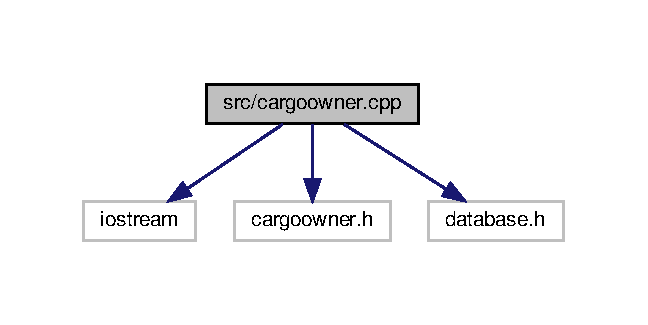
\includegraphics[width=311pt]{cargoowner_8cpp__incl}
\end{center}
\end{figure}
\subsection*{Functions}
\begin{DoxyCompactItemize}
\item 
\mbox{\Hypertarget{cargoowner_8cpp_a7fdc53d1cbb1756de7f8964786ad2fe2}\label{cargoowner_8cpp_a7fdc53d1cbb1756de7f8964786ad2fe2}} 
std\+::string {\bfseries encrypt} (std\+::string pw, std\+::string salt)
\end{DoxyCompactItemize}

\hypertarget{database_8cpp}{}\section{src/database.cpp File Reference}
\label{database_8cpp}\index{src/database.\+cpp@{src/database.\+cpp}}


\hyperlink{classDatabase}{Database} constructor.  


{\ttfamily \#include $<$iostream$>$}\newline
{\ttfamily \#include $<$stdio.\+h$>$}\newline
{\ttfamily \#include \char`\"{}database.\+h\char`\"{}}\newline
{\ttfamily \#include \char`\"{}exception.\+h\char`\"{}}\newline
Include dependency graph for database.\+cpp\+:
\nopagebreak
\begin{figure}[H]
\begin{center}
\leavevmode
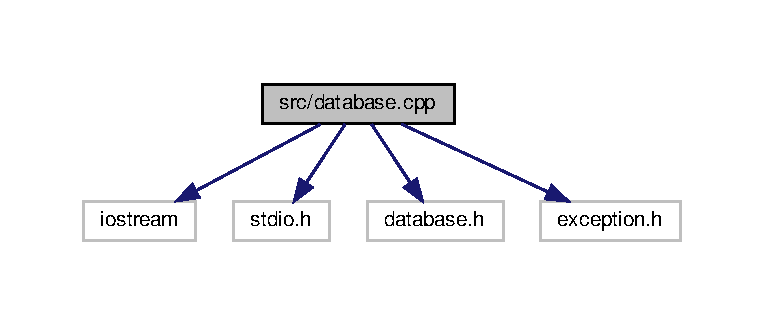
\includegraphics[width=350pt]{database_8cpp__incl}
\end{center}
\end{figure}


\subsection{Detailed Description}
\hyperlink{classDatabase}{Database} constructor. 

Deletes a row from the database.

Returns the database filename.

Creates a new database.

Finds a row in the database.

Writes a row to the database.

Reads a row from the database.

Saves a database.

Loads a database into memory.

\hyperlink{classDatabase}{Database()}

\begin{DoxyAuthor}{Author}
Matthew Boote
\end{DoxyAuthor}

\begin{DoxyParams}[1]{Parameters}
\mbox{\tt in}  & {\em None} & \\
\hline
\mbox{\tt out}  & {\em None} & \\
\hline
\end{DoxyParams}
\begin{DoxyReturn}{Returns}
Boolean None
\end{DoxyReturn}
Load()

\begin{DoxyAuthor}{Author}
Matthew Boote
\end{DoxyAuthor}

\begin{DoxyParams}[1]{Parameters}
\mbox{\tt in}  & {\em std\+::string} & filename\\
\hline
\mbox{\tt out}  & {\em None} & \\
\hline
\end{DoxyParams}
\begin{DoxyReturn}{Returns}
Boolean true or false
\end{DoxyReturn}
Save()

\begin{DoxyAuthor}{Author}
Matthew Boote
\end{DoxyAuthor}

\begin{DoxyParams}[1]{Parameters}
\mbox{\tt in}  & {\em std\+::string} & filename\\
\hline
\end{DoxyParams}
\begin{DoxyReturn}{Returns}
Boolean true or false
\end{DoxyReturn}

\begin{DoxyExceptions}{Exceptions}
{\em Throws} & an error on file I/O error\\
\hline
\end{DoxyExceptions}
Read()

\begin{DoxyAuthor}{Author}
Matthew Boote
\end{DoxyAuthor}
Reads a row of key+values from the database \begin{DoxyVerb}@param[in] std::string key

@param[out] None

@return std::vector<std::string>\end{DoxyVerb}


Write()

\begin{DoxyAuthor}{Author}
Matthew Boote
\end{DoxyAuthor}
Writes a row of key+values to the database \begin{DoxyVerb}@param[in] std::string key,std::vector<std::string> valuevector

@param[out] None

@return std::vector<std::string>\end{DoxyVerb}


Find()

\begin{DoxyAuthor}{Author}
Matthew Boote
\end{DoxyAuthor}
Finds the next row in turn in the database \begin{DoxyVerb}@param[in] None

@param[out] None

@return std::vector<std::string>\end{DoxyVerb}


New()

\begin{DoxyAuthor}{Author}
Matthew Boote
\end{DoxyAuthor}
Creates a database object and corresponding file. \begin{DoxyVerb}@param[in] std::string filename

@param[out] None

@return boolean true or false

@throw Throws on I/O error\end{DoxyVerb}


Get\+File\+Name()

\begin{DoxyAuthor}{Author}
Matthew Boote
\end{DoxyAuthor}

\begin{DoxyParams}[1]{Parameters}
\mbox{\tt in}  & {\em None} & \\
\hline
\mbox{\tt out}  & {\em None} & \\
\hline
\end{DoxyParams}
\begin{DoxyReturn}{Returns}
std\+::string database\+\_\+filename
\end{DoxyReturn}
Delete()

\begin{DoxyAuthor}{Author}
Matthew Boote
\end{DoxyAuthor}
Deletes a row associated with a key \begin{DoxyVerb}@param[in] None

@param[out] None

@return boolean true or false\end{DoxyVerb}

\hypertarget{driver_8cpp}{}\section{src/driver.cpp File Reference}
\label{driver_8cpp}\index{src/driver.\+cpp@{src/driver.\+cpp}}


\hyperlink{classDriver}{Driver} construction.  


{\ttfamily \#include $<$iostream$>$}\newline
{\ttfamily \#include \char`\"{}driver.\+h\char`\"{}}\newline
{\ttfamily \#include \char`\"{}database.\+h\char`\"{}}\newline
{\ttfamily \#include \char`\"{}user.\+h\char`\"{}}\newline
{\ttfamily \#include \char`\"{}transaction.\+h\char`\"{}}\newline
Include dependency graph for driver.\+cpp\+:
\nopagebreak
\begin{figure}[H]
\begin{center}
\leavevmode
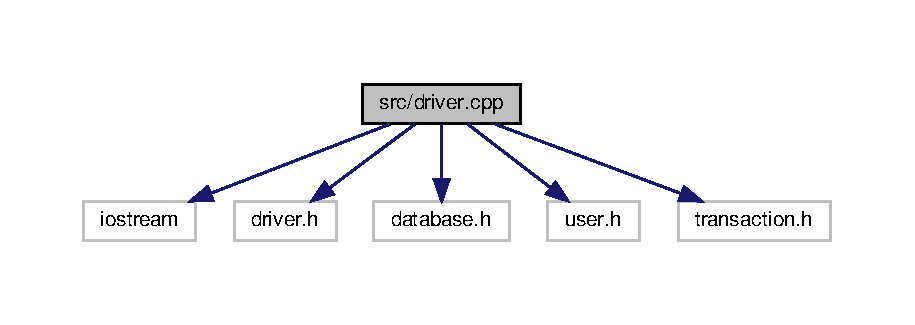
\includegraphics[width=350pt]{driver_8cpp__incl}
\end{center}
\end{figure}
\subsection*{Functions}
\begin{DoxyCompactItemize}
\item 
\mbox{\Hypertarget{driver_8cpp_a7fdc53d1cbb1756de7f8964786ad2fe2}\label{driver_8cpp_a7fdc53d1cbb1756de7f8964786ad2fe2}} 
std\+::string {\bfseries encrypt} (std\+::string pw, std\+::string salt)
\end{DoxyCompactItemize}


\subsection{Detailed Description}
\hyperlink{classDriver}{Driver} construction. 

Sets the driver\textquotesingle{}s C\+PC number.

Validates a driver\textquotesingle{}s C\+PC number.

Gets the driver\textquotesingle{}s driving licence ID number.

Sets the vehicle registration.

Gets the vehicle registration.

Signs up user as a driver.

Finds the nearest driver.

\hyperlink{classDriver}{Driver()}

\begin{DoxyAuthor}{Author}
Matthew Boote
\end{DoxyAuthor}
Loads user database \begin{DoxyVerb}@param[in] None

@param[out] None

@return None\end{DoxyVerb}


Find\+Nearest\+Driver()

\begin{DoxyAuthor}{Author}
Matthew Boote
\end{DoxyAuthor}
The function uses the driver database to find a driver in the same city, province and country. \begin{DoxyVerb}@param[in] std::string city,std::string province,std::string country

@param[out] None

@return Driver object containing information about the driver\end{DoxyVerb}


Sign\+Up\+As\+Driver()

Matthew Boote

Reads user information from cargo owner object into database \begin{DoxyVerb}@param[in] Driver driver

@param[out] None

@return boolean\end{DoxyVerb}


Get\+Registration()

\begin{DoxyAuthor}{Author}
Matthew Boote
\end{DoxyAuthor}

\begin{DoxyParams}[1]{Parameters}
\mbox{\tt in}  & {\em None} & \\
\hline
\mbox{\tt out}  & {\em None} & \\
\hline
\end{DoxyParams}
\begin{DoxyReturn}{Returns}
std\+::string vehicleregistration
\end{DoxyReturn}
Set\+Registration()

\begin{DoxyAuthor}{Author}
Matthew Boote
\end{DoxyAuthor}

\begin{DoxyParams}[1]{Parameters}
\mbox{\tt in}  & {\em \hyperlink{classDriver}{Driver}} & driver\\
\hline
\mbox{\tt out}  & {\em None} & \\
\hline
\end{DoxyParams}
\begin{DoxyReturn}{Returns}
boolean
\end{DoxyReturn}
Get\+Driving\+Licence\+I\+D()

\begin{DoxyAuthor}{Author}
Matthew Boote
\end{DoxyAuthor}

\begin{DoxyParams}[1]{Parameters}
\mbox{\tt in}  & {\em \hyperlink{classDriver}{Driver}} & driver\\
\hline
\mbox{\tt out}  & {\em None} & \\
\hline
\end{DoxyParams}
\begin{DoxyReturn}{Returns}
boolean
\end{DoxyReturn}
Validate\+C\+P\+C()

\begin{DoxyAuthor}{Author}
Matthew Boote
\end{DoxyAuthor}
Checks the C\+PC format and looks up the number in the C\+PC database \begin{DoxyVerb}@param[in] Driver driver

@param[out] None

@return boolean\end{DoxyVerb}


Set\+C\+P\+C()

\begin{DoxyAuthor}{Author}
Matthew Boote
\end{DoxyAuthor}
\begin{DoxyVerb}@param[in] Driver driver

@param[out] None

@return boolean\end{DoxyVerb}

\hypertarget{main_8cpp}{}\section{src/main.cpp File Reference}
\label{main_8cpp}\index{src/main.\+cpp@{src/main.\+cpp}}
{\ttfamily \#include $<$iostream$>$}\newline
{\ttfamily \#include $<$fstream$>$}\newline
{\ttfamily \#include $<$string$>$}\newline
{\ttfamily \#include $<$boost/uuid/uuid.\+hpp$>$}\newline
{\ttfamily \#include $<$boost/uuid/uuid\+\_\+io.\+hpp$>$}\newline
{\ttfamily \#include $<$boost/uuid/random\+\_\+generator.\+hpp$>$}\newline
{\ttfamily \#include $<$boost/lexical\+\_\+cast.\+hpp$>$}\newline
{\ttfamily \#include \char`\"{}main.\+h\char`\"{}}\newline
{\ttfamily \#include \char`\"{}Cargo\+Owner\+User\+Interface.\+h\char`\"{}}\newline
{\ttfamily \#include \char`\"{}Driver\+User\+Interface.\+h\char`\"{}}\newline
{\ttfamily \#include \char`\"{}Transportation\+Company\+User\+Interface.\+h\char`\"{}}\newline
Include dependency graph for main.\+cpp\+:
\nopagebreak
\begin{figure}[H]
\begin{center}
\leavevmode
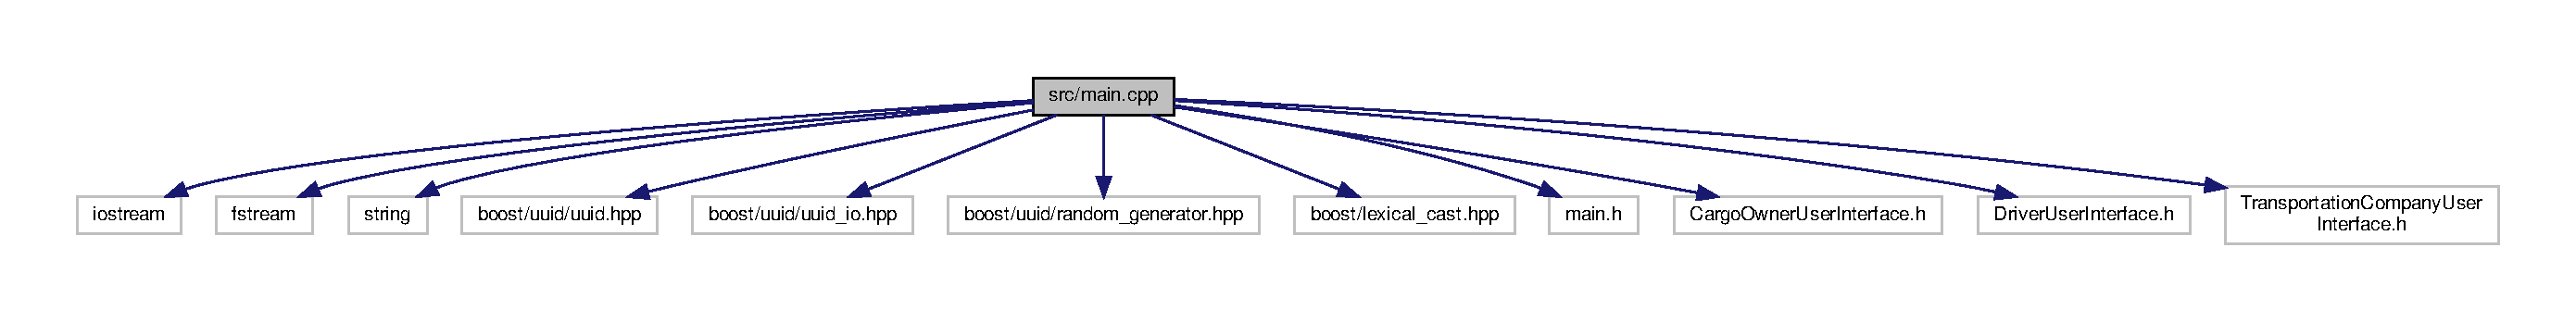
\includegraphics[width=350pt]{main_8cpp__incl}
\end{center}
\end{figure}
\subsection*{Functions}
\begin{DoxyCompactItemize}
\item 
\mbox{\Hypertarget{main_8cpp_ae66f6b31b5ad750f1fe042a706a4e3d4}\label{main_8cpp_ae66f6b31b5ad750f1fe042a706a4e3d4}} 
int {\bfseries main} ()
\end{DoxyCompactItemize}

\hypertarget{transaction_8cpp}{}\section{src/transaction.cpp File Reference}
\label{transaction_8cpp}\index{src/transaction.\+cpp@{src/transaction.\+cpp}}


\hyperlink{classTransaction}{Transaction} constructor.  


{\ttfamily \#include $<$iostream$>$}\newline
{\ttfamily \#include \char`\"{}transaction.\+h\char`\"{}}\newline
{\ttfamily \#include \char`\"{}database.\+h\char`\"{}}\newline
{\ttfamily \#include \char`\"{}Message\+Interface.\+h\char`\"{}}\newline
{\ttfamily \#include \char`\"{}transportationcompany.\+h\char`\"{}}\newline
{\ttfamily \#include $<$boost/uuid/uuid.\+hpp$>$}\newline
{\ttfamily \#include $<$boost/uuid/uuid\+\_\+io.\+hpp$>$}\newline
{\ttfamily \#include $<$boost/uuid/random\+\_\+generator.\+hpp$>$}\newline
{\ttfamily \#include $<$boost/lexical\+\_\+cast.\+hpp$>$}\newline
{\ttfamily \#include \char`\"{}exception.\+h\char`\"{}}\newline
Include dependency graph for transaction.\+cpp\+:
\nopagebreak
\begin{figure}[H]
\begin{center}
\leavevmode
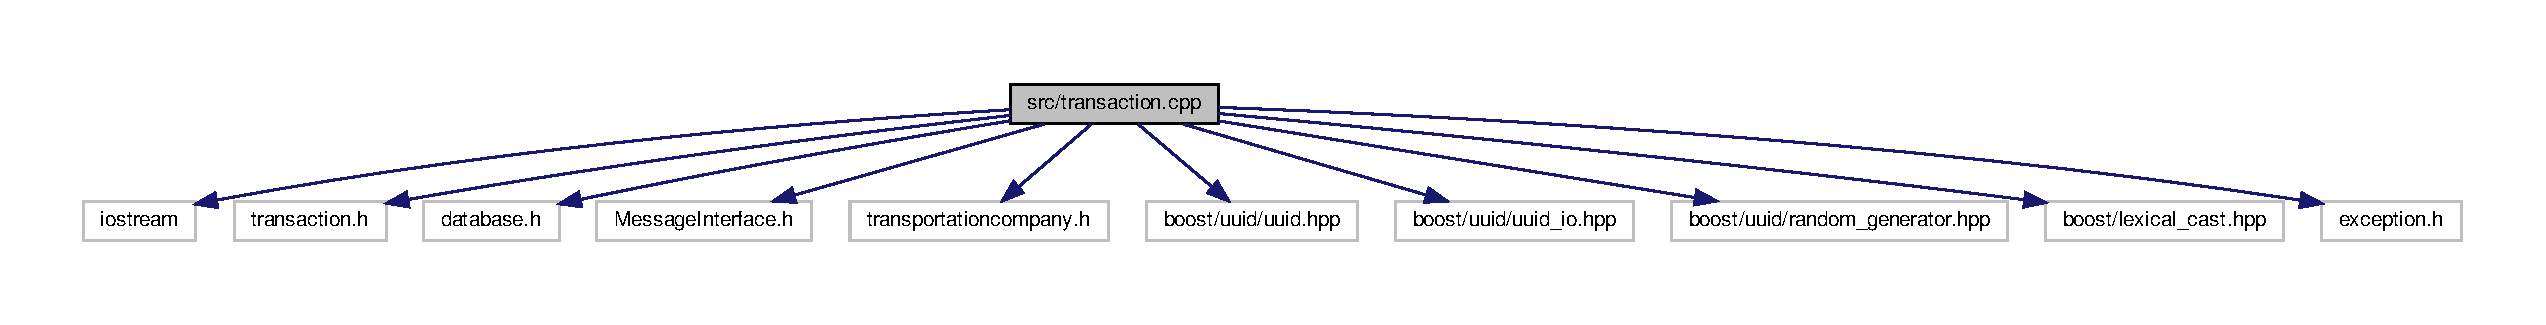
\includegraphics[width=350pt]{transaction_8cpp__incl}
\end{center}
\end{figure}


\subsection{Detailed Description}
\hyperlink{classTransaction}{Transaction} constructor. 

Sets the driver\textquotesingle{}s name.

Gets the driver\textquotesingle{}s name.

Calculates the cost of delivery.

Calculates the driver and transportation company\textquotesingle{}s commission.

Gets the current location.

Sets the order\textquotesingle{}s city.

Sets the order\textquotesingle{}s province.

Sets the order\textquotesingle{}s comments.

Sets the order\textquotesingle{}s description.

Sets the type of the order.

Sets the order\textquotesingle{}s priority.

Sets the order\textquotesingle{}s contact email address.

Sets the order\textquotesingle{}s contact phone number.

Sets the item\textquotesingle{}s weight.

Sets the order\textquotesingle{}s country.

Sets the order\textquotesingle{}s postcode.

Sets the order\textquotesingle{}s delivery address.

Sets the sender\textquotesingle{}s surname.

Sets the sender\textquotesingle{}s first name.

Sets the sender\textquotesingle{}s name.

Sets the order\textquotesingle{}s ID.

Generates a unique boost U\+U\+ID.

Gets the recipient\textquotesingle{}s country.

Gets the order\textquotesingle{}s recipient city.

Gets the order\textquotesingle{}s recipient province.

Gets the order\textquotesingle{}s comment.

Gets the username of the order\textquotesingle{}s recipient.

Gets the weight of the item.

Gets the total cost of the order.

Gets the order\textquotesingle{}s priority.

Gets the email of the order\textquotesingle{}s recipient.

Gets the goods type of the order (Animals, etc)

Gets the order\textquotesingle{}s description.

Gets the order\textquotesingle{}s sender.

Gets the contact phone number of the order\textquotesingle{}s recipient.

Gets the postcode of the order\textquotesingle{}s recipient.

Gets the address of the order\textquotesingle{}s recipient.

Gets the surname of the order\textquotesingle{}s recipient.

Gets the first name of the order\textquotesingle{}s recipient.

Gets the orders ID.

Finds the next transaction in the order databae.

Changes the order\textquotesingle{}s status.

Cancels an order.

Places an order.

\hyperlink{classTransaction}{Transaction()} \begin{DoxyAuthor}{Author}
Matthew Boote
\end{DoxyAuthor}
Initializes transaction object by loading the database associated with the transaction. \begin{DoxyVerb}@param[in] None

@param[out] None

@return None

@throw General exception  \end{DoxyVerb}


Place\+Order() \begin{DoxyAuthor}{Author}
Matthew Boote
\end{DoxyAuthor}
This function adds the order to the user\textquotesingle{}s transaction database, finds the nearest transportation company to the user and sends a message to them. \begin{DoxyVerb}@param[in] std::string senderusername,std::string sendercity,std::string senderprovince,std::string sendercountry

@param[out] None

@return boolean

@throw General exception  \end{DoxyVerb}


Place\+Order() \begin{DoxyAuthor}{Author}
Matthew Boote
\end{DoxyAuthor}
This function deletes the order from the order database. \begin{DoxyVerb}@param[in] std::string senderusername,std::string sendercity,std::string senderprovince,std::string sendercountry

@param[out] None

@return boolean\end{DoxyVerb}


Change\+Status() \begin{DoxyAuthor}{Author}
Matthew Boote
\end{DoxyAuthor}
This function changes the order status in the order\textquotesingle{}s database entry. Order status can be waiting, on road and delivered. \begin{DoxyVerb}@param[in] uuid orderid,std::string status

@param[out] None

@return boolean

@throw General exception  \end{DoxyVerb}


Find\+Next\+Transaction() \begin{DoxyAuthor}{Author}
Matthew Boote
\end{DoxyAuthor}
This function returns each order in the database, in sequence. \begin{DoxyVerb}@param[in] None

@param[out] None

@return boolean

@throw Throws error if database entry not found\end{DoxyVerb}


Get\+I\+D() \begin{DoxyAuthor}{Author}
Matthew Boote
\end{DoxyAuthor}

\begin{DoxyParams}[1]{Parameters}
\mbox{\tt in}  & {\em None} & \\
\hline
\mbox{\tt out}  & {\em None} & \\
\hline
\end{DoxyParams}
\begin{DoxyReturn}{Returns}
uuid ID
\end{DoxyReturn}
Get\+First\+Name() \begin{DoxyAuthor}{Author}
Matthew Boote
\end{DoxyAuthor}

\begin{DoxyParams}[1]{Parameters}
\mbox{\tt in}  & {\em None} & \\
\hline
\mbox{\tt out}  & {\em None} & \\
\hline
\end{DoxyParams}
\begin{DoxyReturn}{Returns}
uuid ID
\end{DoxyReturn}
Get\+First\+Name() \begin{DoxyAuthor}{Author}
Matthew Boote
\end{DoxyAuthor}

\begin{DoxyParams}[1]{Parameters}
\mbox{\tt in}  & {\em None} & \\
\hline
\mbox{\tt out}  & {\em None} & \\
\hline
\end{DoxyParams}
\begin{DoxyReturn}{Returns}
std\+::string
\end{DoxyReturn}
Get\+Delivery\+Address() \begin{DoxyAuthor}{Author}
Matthew Boote
\end{DoxyAuthor}

\begin{DoxyParams}[1]{Parameters}
\mbox{\tt in}  & {\em None} & \\
\hline
\mbox{\tt out}  & {\em None} & \\
\hline
\end{DoxyParams}
\begin{DoxyReturn}{Returns}
std\+::string
\end{DoxyReturn}
Get\+Post\+Code() \begin{DoxyAuthor}{Author}
Matthew Boote
\end{DoxyAuthor}

\begin{DoxyParams}[1]{Parameters}
\mbox{\tt in}  & {\em None} & \\
\hline
\mbox{\tt out}  & {\em None} & \\
\hline
\end{DoxyParams}
\begin{DoxyReturn}{Returns}
std\+::string
\end{DoxyReturn}
Get\+Contat\+Phone() \begin{DoxyAuthor}{Author}
Matthew Boote
\end{DoxyAuthor}

\begin{DoxyParams}[1]{Parameters}
\mbox{\tt in}  & {\em None} & \\
\hline
\mbox{\tt out}  & {\em None} & \\
\hline
\end{DoxyParams}
\begin{DoxyReturn}{Returns}
std\+::string
\end{DoxyReturn}
Get\+Sender() \begin{DoxyAuthor}{Author}
Matthew Boote
\end{DoxyAuthor}

\begin{DoxyParams}[1]{Parameters}
\mbox{\tt in}  & {\em None} & \\
\hline
\mbox{\tt out}  & {\em None} & \\
\hline
\end{DoxyParams}
\begin{DoxyReturn}{Returns}
std\+::string
\end{DoxyReturn}
Get\+Priority() \begin{DoxyAuthor}{Author}
Matthew Boote
\end{DoxyAuthor}

\begin{DoxyParams}[1]{Parameters}
\mbox{\tt in}  & {\em None} & \\
\hline
\mbox{\tt out}  & {\em None} & \\
\hline
\end{DoxyParams}
\begin{DoxyReturn}{Returns}
int
\end{DoxyReturn}
Get\+Total\+Cost() \begin{DoxyAuthor}{Author}
Matthew Boote
\end{DoxyAuthor}
The order is calculated from the distance, weight and the driver and transportation company\textquotesingle{}s commission.


\begin{DoxyParams}[1]{Parameters}
\mbox{\tt in}  & {\em None} & \\
\hline
\mbox{\tt out}  & {\em None} & \\
\hline
\end{DoxyParams}
\begin{DoxyReturn}{Returns}
double
\end{DoxyReturn}
Get\+Item\+Weight() \begin{DoxyAuthor}{Author}
Matthew Boote
\end{DoxyAuthor}

\begin{DoxyParams}[1]{Parameters}
\mbox{\tt in}  & {\em None} & \\
\hline
\mbox{\tt out}  & {\em None} & \\
\hline
\end{DoxyParams}
\begin{DoxyReturn}{Returns}
double
\end{DoxyReturn}
Get\+Recipient\+Username() \begin{DoxyAuthor}{Author}
Matthew Boote
\end{DoxyAuthor}

\begin{DoxyParams}[1]{Parameters}
\mbox{\tt in}  & {\em None} & \\
\hline
\mbox{\tt out}  & {\em None} & \\
\hline
\end{DoxyParams}
\begin{DoxyReturn}{Returns}
std\+::string
\end{DoxyReturn}
Get\+Province() \begin{DoxyAuthor}{Author}
Matthew Boote
\end{DoxyAuthor}

\begin{DoxyParams}[1]{Parameters}
\mbox{\tt in}  & {\em None} & \\
\hline
\mbox{\tt out}  & {\em None} & \\
\hline
\end{DoxyParams}
\begin{DoxyReturn}{Returns}
std\+::string
\end{DoxyReturn}
Get\+Country() \begin{DoxyAuthor}{Author}
Matthew Boote
\end{DoxyAuthor}

\begin{DoxyParams}[1]{Parameters}
\mbox{\tt in}  & {\em None} & \\
\hline
\mbox{\tt out}  & {\em None} & \\
\hline
\end{DoxyParams}
\begin{DoxyReturn}{Returns}
std\+::string
\end{DoxyReturn}
Generate\+I\+D() \begin{DoxyAuthor}{Author}
Matthew Boote
\end{DoxyAuthor}
The ID is used as the primary key for the order database


\begin{DoxyParams}[1]{Parameters}
\mbox{\tt in}  & {\em None} & \\
\hline
\mbox{\tt out}  & {\em None} & \\
\hline
\end{DoxyParams}
\begin{DoxyReturn}{Returns}
None
\end{DoxyReturn}
Set\+I\+D() \begin{DoxyAuthor}{Author}
Matthew Boote
\end{DoxyAuthor}
The ID is used as the primary key for the order database


\begin{DoxyParams}[1]{Parameters}
\mbox{\tt in}  & {\em uuid} & id\\
\hline
\mbox{\tt out}  & {\em None} & \\
\hline
\end{DoxyParams}
\begin{DoxyReturn}{Returns}
None
\end{DoxyReturn}
Set\+Sender() \begin{DoxyAuthor}{Author}
Matthew Boote
\end{DoxyAuthor}

\begin{DoxyParams}[1]{Parameters}
\mbox{\tt in}  & {\em std\+::string} & fname\\
\hline
\mbox{\tt out}  & {\em None} & \\
\hline
\end{DoxyParams}
\begin{DoxyReturn}{Returns}
std\+::string
\end{DoxyReturn}
Set\+Sender\+First\+Name() \begin{DoxyAuthor}{Author}
Matthew Boote
\end{DoxyAuthor}

\begin{DoxyParams}[1]{Parameters}
\mbox{\tt in}  & {\em std\+::string} & fname\\
\hline
\mbox{\tt out}  & {\em None} & \\
\hline
\end{DoxyParams}
\begin{DoxyReturn}{Returns}
None
\end{DoxyReturn}
Set\+Sender\+Surname() \begin{DoxyAuthor}{Author}
Matthew Boote
\end{DoxyAuthor}

\begin{DoxyParams}[1]{Parameters}
\mbox{\tt in}  & {\em std\+::string} & sname\\
\hline
\mbox{\tt out}  & {\em None} & \\
\hline
\end{DoxyParams}
\begin{DoxyReturn}{Returns}
None
\end{DoxyReturn}
Set\+Sender() \begin{DoxyAuthor}{Author}
Matthew Boote
\end{DoxyAuthor}

\begin{DoxyParams}[1]{Parameters}
\mbox{\tt in}  & {\em std\+::string} & address\\
\hline
\mbox{\tt out}  & {\em None} & \\
\hline
\end{DoxyParams}
\begin{DoxyReturn}{Returns}
None
\end{DoxyReturn}
Set\+Post\+Code() \begin{DoxyAuthor}{Author}
Matthew Boote
\end{DoxyAuthor}

\begin{DoxyParams}[1]{Parameters}
\mbox{\tt in}  & {\em std\+::string} & pcode\\
\hline
\mbox{\tt out}  & {\em None} & \\
\hline
\end{DoxyParams}
\begin{DoxyReturn}{Returns}
None
\end{DoxyReturn}
Set\+Sender() \begin{DoxyAuthor}{Author}
Matthew Boote
\end{DoxyAuthor}

\begin{DoxyParams}[1]{Parameters}
\mbox{\tt in}  & {\em std\+::string} & country\\
\hline
\mbox{\tt out}  & {\em None} & \\
\hline
\end{DoxyParams}
\begin{DoxyReturn}{Returns}
None
\end{DoxyReturn}
Set\+Weight() \begin{DoxyAuthor}{Author}
Matthew Boote
\end{DoxyAuthor}

\begin{DoxyParams}[1]{Parameters}
\mbox{\tt in}  & {\em double} & w\\
\hline
\mbox{\tt out}  & {\em None} & \\
\hline
\end{DoxyParams}
\begin{DoxyReturn}{Returns}
None
\end{DoxyReturn}
Set\+Contact\+Phone() \begin{DoxyAuthor}{Author}
Matthew Boote
\end{DoxyAuthor}

\begin{DoxyParams}[1]{Parameters}
\mbox{\tt in}  & {\em std\+::string} & pnumber\\
\hline
\mbox{\tt out}  & {\em None} & \\
\hline
\end{DoxyParams}
\begin{DoxyReturn}{Returns}
None
\end{DoxyReturn}
Set\+Contact\+Email() \begin{DoxyAuthor}{Author}
Matthew Boote
\end{DoxyAuthor}

\begin{DoxyParams}[1]{Parameters}
\mbox{\tt in}  & {\em std\+::string} & email\\
\hline
\mbox{\tt out}  & {\em None} & \\
\hline
\end{DoxyParams}
\begin{DoxyReturn}{Returns}
None
\end{DoxyReturn}
Set\+Priority() \begin{DoxyAuthor}{Author}
Matthew Boote
\end{DoxyAuthor}
The priority is from 1-\/3 and determines the speed and cost of the delivery.


\begin{DoxyParams}[1]{Parameters}
\mbox{\tt in}  & {\em std\+::string} & pnumber\\
\hline
\mbox{\tt out}  & {\em None} & \\
\hline
\end{DoxyParams}
\begin{DoxyReturn}{Returns}
None
\end{DoxyReturn}
Set\+Goods\+Type() \begin{DoxyAuthor}{Author}
Matthew Boote
\end{DoxyAuthor}

\begin{DoxyParams}[1]{Parameters}
\mbox{\tt in}  & {\em std\+::string} & type\\
\hline
\mbox{\tt out}  & {\em None} & \\
\hline
\end{DoxyParams}
\begin{DoxyReturn}{Returns}
None
\end{DoxyReturn}
Set\+Description() \begin{DoxyAuthor}{Author}
Matthew Boote
\end{DoxyAuthor}

\begin{DoxyParams}[1]{Parameters}
\mbox{\tt in}  & {\em std\+::string} & desc\\
\hline
\mbox{\tt out}  & {\em None} & \\
\hline
\end{DoxyParams}
\begin{DoxyReturn}{Returns}
None
\end{DoxyReturn}
Set\+Coments() \begin{DoxyAuthor}{Author}
Matthew Boote
\end{DoxyAuthor}

\begin{DoxyParams}[1]{Parameters}
\mbox{\tt in}  & {\em std\+::string} & comments\\
\hline
\mbox{\tt out}  & {\em None} & \\
\hline
\end{DoxyParams}
\begin{DoxyReturn}{Returns}
None
\end{DoxyReturn}
Set\+Province() \begin{DoxyAuthor}{Author}
Matthew Boote
\end{DoxyAuthor}

\begin{DoxyParams}[1]{Parameters}
\mbox{\tt in}  & {\em std\+::string} & pnumber\\
\hline
\mbox{\tt out}  & {\em None} & \\
\hline
\end{DoxyParams}
\begin{DoxyReturn}{Returns}
None
\end{DoxyReturn}
Set\+City() \begin{DoxyAuthor}{Author}
Matthew Boote
\end{DoxyAuthor}

\begin{DoxyParams}[1]{Parameters}
\mbox{\tt in}  & {\em std\+::string} & pnumber\\
\hline
\mbox{\tt out}  & {\em None} & \\
\hline
\end{DoxyParams}
\begin{DoxyReturn}{Returns}
None
\end{DoxyReturn}
Set\+Location() \begin{DoxyAuthor}{Author}
Matthew Boote
\end{DoxyAuthor}

\begin{DoxyParams}[1]{Parameters}
\mbox{\tt in}  & {\em None} & \\
\hline
\mbox{\tt out}  & {\em None} & \\
\hline
\end{DoxyParams}
\begin{DoxyReturn}{Returns}
std\+::vector$<$double$>$
\end{DoxyReturn}
Calculate\+Commission() \begin{DoxyAuthor}{Author}
Matthew Boote
\end{DoxyAuthor}

\begin{DoxyParams}[1]{Parameters}
\mbox{\tt in}  & {\em None} & \\
\hline
\mbox{\tt out}  & {\em None} & \\
\hline
\end{DoxyParams}
\begin{DoxyReturn}{Returns}
std\+::vector$<$double$>$
\end{DoxyReturn}
Calculate\+Shipping\+Rates() Calculates the shipping rate for the order

\begin{DoxyAuthor}{Author}
Matthew Boote
\end{DoxyAuthor}
The shipping rate is calculated from the distance the order is to travel and the weight of the item.


\begin{DoxyParams}[1]{Parameters}
\mbox{\tt in}  & {\em None} & \\
\hline
\mbox{\tt out}  & {\em None} & \\
\hline
\end{DoxyParams}
\begin{DoxyReturn}{Returns}
std\+::vector$<$double$>$
\end{DoxyReturn}
Calculate\+Cost\+Of\+Delivery() \begin{DoxyAuthor}{Author}
Matthew Boote
\end{DoxyAuthor}
the cost of delivery is (shipping rates+commission)$\ast$priority 
\begin{DoxyParams}[1]{Parameters}
\mbox{\tt in}  & {\em None} & \\
\hline
\mbox{\tt out}  & {\em None} & \\
\hline
\end{DoxyParams}
\begin{DoxyReturn}{Returns}
std\+::vector$<$double$>$
\end{DoxyReturn}
Get\+Driver\+Name() \begin{DoxyAuthor}{Author}
Matthew Boote
\end{DoxyAuthor}

\begin{DoxyParams}[1]{Parameters}
\mbox{\tt in}  & {\em None} & \\
\hline
\mbox{\tt out}  & {\em None} & \\
\hline
\end{DoxyParams}
\begin{DoxyReturn}{Returns}
std\+::string
\end{DoxyReturn}
Set\+Driver\+Name() \begin{DoxyAuthor}{Author}
Matthew Boote
\end{DoxyAuthor}

\begin{DoxyParams}[1]{Parameters}
\mbox{\tt in}  & {\em std\+::string} & drivername\\
\hline
\mbox{\tt out}  & {\em None} & \\
\hline
\end{DoxyParams}
\begin{DoxyReturn}{Returns}
None 
\end{DoxyReturn}

\hypertarget{transportationcompany_8cpp}{}\section{src/transportationcompany.cpp File Reference}
\label{transportationcompany_8cpp}\index{src/transportationcompany.\+cpp@{src/transportationcompany.\+cpp}}


Transportation\+Company constructor.  


{\ttfamily \#include $<$string$>$}\newline
{\ttfamily \#include $<$sstream$>$}\newline
{\ttfamily \#include $<$math.\+h$>$}\newline
{\ttfamily \#include \char`\"{}user.\+h\char`\"{}}\newline
{\ttfamily \#include \char`\"{}transportationcompany.\+h\char`\"{}}\newline
{\ttfamily \#include \char`\"{}database.\+h\char`\"{}}\newline
Include dependency graph for transportationcompany.\+cpp\+:
\nopagebreak
\begin{figure}[H]
\begin{center}
\leavevmode
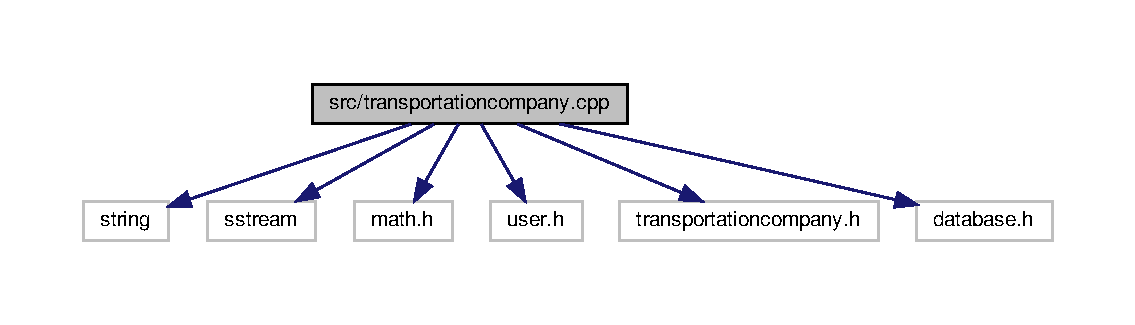
\includegraphics[width=350pt]{transportationcompany_8cpp__incl}
\end{center}
\end{figure}


\subsection{Detailed Description}
Transportation\+Company constructor. 

Gets the type of goods the transportation company transports.

Sets the type of goods the transportation company transports.

Finds the nearest transportation company.

Sets the company name.

Signs up as a transportation company.

Signs up as a cargo owner.

Transportation\+Company() \begin{DoxyAuthor}{Author}
Matthew Boote
\end{DoxyAuthor}
Initializes transportation company object by loading Users database \begin{DoxyVerb}@param[in] None

@param[out] None

@return None\end{DoxyVerb}


Sign\+Up\+As\+Transportation Company()

\begin{DoxyAuthor}{Author}
Matthew Boote
\end{DoxyAuthor}
Reads user information from cargo owner object into database \begin{DoxyVerb}@param[in] Transportation Company cargowner     Cargo owner object

@param[out] None

@return Boolean true or false\end{DoxyVerb}


Get\+Company\+Name()

\begin{DoxyAuthor}{Author}
Matthew Boote
\end{DoxyAuthor}
Reads user information from transportation into database. This function is called from the sign up user interface. \begin{DoxyVerb}@param[in] None

@param[out] None

@return std::string CompanyName\end{DoxyVerb}


Set\+Company\+Name()

\begin{DoxyAuthor}{Author}
Matthew Boote
\end{DoxyAuthor}

\begin{DoxyParams}[1]{Parameters}
\mbox{\tt in}  & {\em std\+::string} & companyname\\
\hline
\mbox{\tt out}  & {\em None} & \\
\hline
\end{DoxyParams}
\begin{DoxyReturn}{Returns}
None
\end{DoxyReturn}
Find\+Nearest\+Transportation\+Company()

\begin{DoxyAuthor}{Author}
Matthew Boote
\end{DoxyAuthor}
Searches the database for a transportation company that is in the same city,province and country \begin{DoxyVerb}@param[in] std::string city,std::string province,std::string country

@param[out] None

@return TransportationCompany object\end{DoxyVerb}


Set\+Goods\+Transportation\+Type()

\begin{DoxyAuthor}{Author}
Matthew Boote
\end{DoxyAuthor}
\begin{DoxyVerb}@param[in] std::string GoodsType

@param[out] None

@return None\end{DoxyVerb}


Get\+Goods\+Transportation\+Type()

\begin{DoxyAuthor}{Author}
Matthew Boote
\end{DoxyAuthor}

\begin{DoxyParams}[1]{Parameters}
\mbox{\tt in}  & {\em None} & \\
\hline
\mbox{\tt out}  & {\em None} & \\
\hline
\end{DoxyParams}
\begin{DoxyReturn}{Returns}
std\+::string goodstype 
\end{DoxyReturn}

\hypertarget{user_8cpp}{}\section{src/user.cpp File Reference}
\label{user_8cpp}\index{src/user.\+cpp@{src/user.\+cpp}}


\hyperlink{classUser}{User} constructor.  


{\ttfamily \#include $<$iostream$>$}\newline
{\ttfamily \#include $<$cstring$>$}\newline
{\ttfamily \#include $<$string$>$}\newline
{\ttfamily \#include \char`\"{}user.\+h\char`\"{}}\newline
{\ttfamily \#include \char`\"{}crypt.\+h\char`\"{}}\newline
{\ttfamily \#include \char`\"{}exception.\+h\char`\"{}}\newline
{\ttfamily \#include $<$stdio.\+h$>$}\newline
Include dependency graph for user.\+cpp\+:
\nopagebreak
\begin{figure}[H]
\begin{center}
\leavevmode
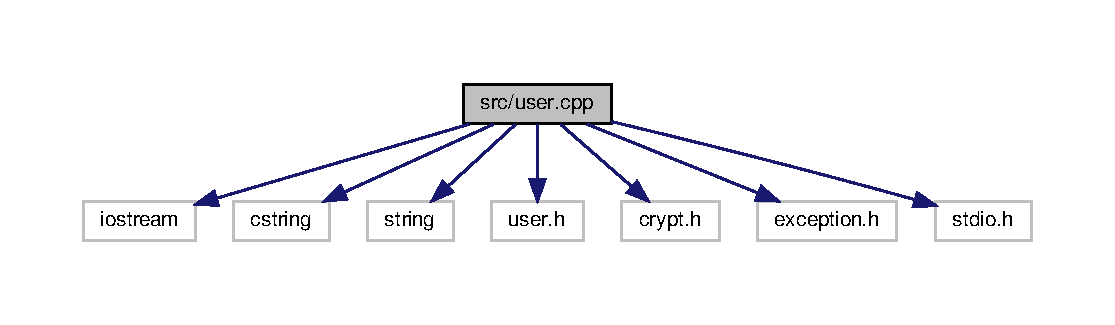
\includegraphics[width=350pt]{user_8cpp__incl}
\end{center}
\end{figure}


\subsection{Detailed Description}
\hyperlink{classUser}{User} constructor. 

Sets the National Insurance number.

Sets the National Insurance number of the user.

Hashes the password.

Signs the user out.

Signs in a user.

Sets the account type of the user.

Sets the country of the user.

Sets the province of the user.

Sets the city of the user.

Sets the email address of the user.

Sets the phone number of the user.

Sets the address of the user.

Sets the first name of the user.

Sets the password.

Sets the username.

Gets the type of account.

Gets user\textquotesingle{}s country.

Gets email address.

Gets phone number.

Gets postcode.

Gets province.

Gets city.

Gets address.

Gets surname.

Gets first name of user.

Gets password.

Gets username.

\hyperlink{classUser}{User()}

\begin{DoxyAuthor}{Author}
Matthew Boote
\end{DoxyAuthor}
Creates new database object \begin{DoxyVerb}@param[in] std::string cname        Company name

@param[out] None

@return None\end{DoxyVerb}


Get\+Username()

\begin{DoxyAuthor}{Author}
Matthew Boote
\end{DoxyAuthor}
Gets username attribute \begin{DoxyVerb}@param[in] None

@param[out] None

@return std::string company name\end{DoxyVerb}


Get\+Password()

\begin{DoxyAuthor}{Author}
Matthew Boote
\end{DoxyAuthor}
Gets password from user object \begin{DoxyVerb}@param[in] None

@param[out] None

@return std::string password\end{DoxyVerb}


Get\+Firstname()

\begin{DoxyAuthor}{Author}
Matthew Boote
\end{DoxyAuthor}
Gets first name from object \begin{DoxyVerb}@param[in] None

@param[out] None

@return std::string firstname\end{DoxyVerb}


Get\+Surname()

\begin{DoxyAuthor}{Author}
Matthew Boote
\end{DoxyAuthor}
Gets surname from user object \begin{DoxyVerb}@param[in] None

@param[out] None

@return std::string surname\end{DoxyVerb}


Get\+Address()

\begin{DoxyAuthor}{Author}
Matthew Boote
\end{DoxyAuthor}
Gets address from user object \begin{DoxyVerb}@param[in] None

@param[out] None

@return std::string address\end{DoxyVerb}


Get\+City()

\begin{DoxyAuthor}{Author}
Matthew Boote
\end{DoxyAuthor}
Gets city from user object \begin{DoxyVerb}@param[in] None

@param[out] None

@return std::string city\end{DoxyVerb}


Get\+Province()

\begin{DoxyAuthor}{Author}
Matthew Boote
\end{DoxyAuthor}
Gets province from user object \begin{DoxyVerb}@param[in] None

@param[out] None

@return std::string province\end{DoxyVerb}


Get\+Postcode()

\begin{DoxyAuthor}{Author}
Matthew Boote
\end{DoxyAuthor}
Gets postcode from user object \begin{DoxyVerb}@param[in] None

@param[out] None

@return std::string postcode\end{DoxyVerb}


Get\+Province()

\begin{DoxyAuthor}{Author}
Matthew Boote
\end{DoxyAuthor}
Gets phone number from user object \begin{DoxyVerb}@param[in] None

@param[out] None

@return std::string phonenumber\end{DoxyVerb}


Get\+Email()

\begin{DoxyAuthor}{Author}
Matthew Boote
\end{DoxyAuthor}
Gets email address from user object \begin{DoxyVerb}@param[in] None

@param[out] None

@return std::string email\end{DoxyVerb}


Get\+Country()

\begin{DoxyAuthor}{Author}
Matthew Boote
\end{DoxyAuthor}
Gets country from user object \begin{DoxyVerb}@param[in] None

@param[out] None

@return std::string country\end{DoxyVerb}


Get\+Province()

\begin{DoxyAuthor}{Author}
Matthew Boote
\end{DoxyAuthor}
Gets the type of user (\hyperlink{classCargoOwner}{Cargo\+Owner}, \hyperlink{classDriver}{Driver} or Transportation\+Company) \begin{DoxyVerb}@param[in] None

@param[out] None

@return std::string usertype\end{DoxyVerb}


Set\+Username()

\begin{DoxyAuthor}{Author}
Matthew Boote
\end{DoxyAuthor}
Sets the username in the object \begin{DoxyVerb}@param[in] std::string username

@param[out] None

@return None\end{DoxyVerb}


Set\+Password()

\begin{DoxyAuthor}{Author}
Matthew Boote
\end{DoxyAuthor}
Sets the password in the object \begin{DoxyVerb}@param[in] std::string password

@param[out] None

@return None\end{DoxyVerb}


Set\+Firstname()

\begin{DoxyAuthor}{Author}
Matthew Boote
\end{DoxyAuthor}
Sets the first name in the object \begin{DoxyVerb}@param[in] std::string user

@param[out] None

@return None\end{DoxyVerb}


Set\+Surname()

\begin{DoxyAuthor}{Author}
Matthew Boote
\end{DoxyAuthor}
Sets the first name in the object/ \begin{DoxyVerb}@param[in] std::string sname

@param[out] None

@return None\end{DoxyVerb}


Set\+Address()

\begin{DoxyAuthor}{Author}
Matthew Boote
\end{DoxyAuthor}
Sets the address in the object \begin{DoxyVerb}@param[in] std::string user

@param[out] None

@return None\end{DoxyVerb}


Set\+Firstname()

\begin{DoxyAuthor}{Author}
Matthew Boote
\end{DoxyAuthor}
Sets the first name in the object/ \begin{DoxyVerb}@param[in] std::string user

@param[out] None

@return None\end{DoxyVerb}


Set\+Firstname()

\begin{DoxyAuthor}{Author}
Matthew Boote
\end{DoxyAuthor}
Sets the phone number in the object/ \begin{DoxyVerb}@param[in] std::string phonenumber

@param[out] None

@return None\end{DoxyVerb}


Set\+Email()

\begin{DoxyAuthor}{Author}
Matthew Boote
\end{DoxyAuthor}
Sets the email address in the object/ \begin{DoxyVerb}@param[in] std::string emailaddress

@param[out] None

@return None\end{DoxyVerb}


Set\+City()

\begin{DoxyAuthor}{Author}
Matthew Boote
\end{DoxyAuthor}
Sets the city in the object \begin{DoxyVerb}@param[in] std::string newcity

@param[out] None

@return None\end{DoxyVerb}


Set\+Province()

\begin{DoxyAuthor}{Author}
Matthew Boote
\end{DoxyAuthor}
Sets the province in the object \begin{DoxyVerb}@param[in] std::string newprovince

@param[out] None

@return None\end{DoxyVerb}


Set\+Country()

\begin{DoxyAuthor}{Author}
Matthew Boote
\end{DoxyAuthor}
Sets the country in the object \begin{DoxyVerb}@param[in] std::string state

@param[out] None

@return None\end{DoxyVerb}


Set\+Account\+Type()

\begin{DoxyAuthor}{Author}
Matthew Boote
\end{DoxyAuthor}
Sets the account type (\hyperlink{classCargoOwner}{Cargo\+Owner}, \hyperlink{classDriver}{Driver}, Transportation\+Company) \begin{DoxyVerb}@param[in] std::string atype

@param[out] None

@return None\end{DoxyVerb}


Sign\+In()

\begin{DoxyAuthor}{Author}
Matthew Boote
\end{DoxyAuthor}
Sign\+In user reads the user account details from the user database, and compares them to the username and password. If the username and password match, it loads the information into the object. \begin{DoxyVerb}@param[in] std::string user

@param[out] None

@return true or false\end{DoxyVerb}


Sign\+Out()

\begin{DoxyAuthor}{Author}
Matthew Boote
\end{DoxyAuthor}
Signs the user out \begin{DoxyVerb}@param[in] None

@param[out] None

@return boolean\end{DoxyVerb}


Hash\+Password

\begin{DoxyAuthor}{Author}
Matthew Boote
\end{DoxyAuthor}
The function hash the password with the U\+N\+IX crypt() function using the username as the salt. It converts the salt and password to char $\ast$, hashes the password and converts it back \begin{DoxyVerb}@param[in] std::string salt,std::string password

@param[out] None

@return None\end{DoxyVerb}


Set\+N\+I\+Number()

\begin{DoxyAuthor}{Author}
Matthew Boote
\end{DoxyAuthor}

\begin{DoxyParams}[1]{Parameters}
\mbox{\tt in}  & {\em std\+::string} & ni\\
\hline
\mbox{\tt out}  & {\em None} & \\
\hline
\end{DoxyParams}
\begin{DoxyReturn}{Returns}
None
\end{DoxyReturn}
Get\+N\+I\+Number()

\begin{DoxyAuthor}{Author}
Matthew Boote
\end{DoxyAuthor}

\begin{DoxyParams}[1]{Parameters}
\mbox{\tt in}  & {\em std\+::string} & user\\
\hline
\mbox{\tt out}  & {\em None} & \\
\hline
\end{DoxyParams}
\begin{DoxyReturn}{Returns}
None 
\end{DoxyReturn}

\hypertarget{vehicle_8cpp}{}\section{src/vehicle.cpp File Reference}
\label{vehicle_8cpp}\index{src/vehicle.\+cpp@{src/vehicle.\+cpp}}


\hyperlink{classVehicle}{Vehicle} constructor.  


{\ttfamily \#include $<$iostream$>$}\newline
{\ttfamily \#include \char`\"{}vehicle.\+h\char`\"{}}\newline
{\ttfamily \#include \char`\"{}database.\+h\char`\"{}}\newline
Include dependency graph for vehicle.\+cpp\+:
\nopagebreak
\begin{figure}[H]
\begin{center}
\leavevmode
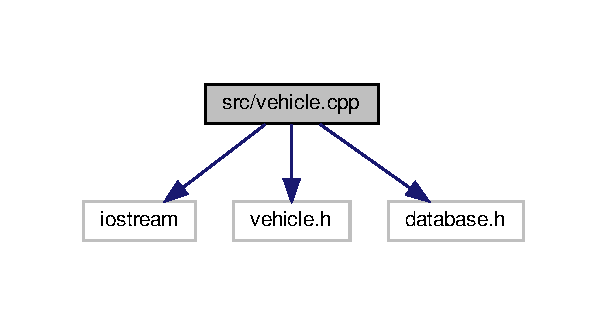
\includegraphics[width=292pt]{vehicle_8cpp__incl}
\end{center}
\end{figure}
\subsection*{Variables}
\begin{DoxyCompactItemize}
\item 
\mbox{\Hypertarget{vehicle_8cpp_ae2fa874a15922b9f12b4f26e0905f526}\label{vehicle_8cpp_ae2fa874a15922b9f12b4f26e0905f526}} 
\hyperlink{classDatabase}{Database} $\ast$ {\bfseries Vehicle\+Database}
\end{DoxyCompactItemize}


\subsection{Detailed Description}
\hyperlink{classVehicle}{Vehicle} constructor. 

Validates vehicle registration.

Sets the vehicle height.

Sets the vehicle weight.

Sets the vehicle type.

Sets the vehicle registration.

Get\+Height.

Get vehicle weight.

Gets the vehicle type.

Gets the vehicle registration number.

Adds a vehicle to the vehicle database.

\hyperlink{classVehicle}{Vehicle()}

\begin{DoxyAuthor}{Author}
Matthew Boote
\end{DoxyAuthor}
Creates a vehicle object. Loads the vehicle database \begin{DoxyVerb}@param[in] None

@param[out] None

@return None\end{DoxyVerb}


Add\+Vehicle()

\begin{DoxyAuthor}{Author}
Matthew Boote
\end{DoxyAuthor}

\begin{DoxyParams}[1]{Parameters}
\mbox{\tt in}  & {\em \hyperlink{classVehicle}{Vehicle}} & vehicle\\
\hline
\mbox{\tt out}  & {\em None} & \\
\hline
\end{DoxyParams}
\begin{DoxyReturn}{Returns}
boolean
\end{DoxyReturn}
Get\+Registration()

\begin{DoxyAuthor}{Author}
Matthew Boote
\end{DoxyAuthor}

\begin{DoxyParams}[1]{Parameters}
\mbox{\tt in}  & {\em None} & \\
\hline
\mbox{\tt out}  & {\em None} & \\
\hline
\end{DoxyParams}
\begin{DoxyReturn}{Returns}
std\+::string
\end{DoxyReturn}
Get\+Vehicle\+Type()

\begin{DoxyAuthor}{Author}
Matthew Boote
\end{DoxyAuthor}

\begin{DoxyParams}[1]{Parameters}
\mbox{\tt in}  & {\em std\+::string} & cname Company name\\
\hline
\mbox{\tt out}  & {\em None} & \\
\hline
\end{DoxyParams}
\begin{DoxyReturn}{Returns}
std\+::string
\end{DoxyReturn}
Get\+Weight()

\begin{DoxyAuthor}{Author}
Matthew Boote
\end{DoxyAuthor}

\begin{DoxyParams}[1]{Parameters}
\mbox{\tt in}  & {\em None} & \\
\hline
\mbox{\tt out}  & {\em None} & \\
\hline
\end{DoxyParams}
\begin{DoxyReturn}{Returns}
double
\end{DoxyReturn}
\hyperlink{classUser}{User()}

\begin{DoxyAuthor}{Author}
Matthew Boote
\end{DoxyAuthor}
Gets the vehicle height \begin{DoxyVerb}@param[in] None

@param[out] None

@return double\end{DoxyVerb}


Set\+Registration()

\begin{DoxyAuthor}{Author}
Matthew Boote
\end{DoxyAuthor}

\begin{DoxyParams}[1]{Parameters}
\mbox{\tt in}  & {\em std\+::string} & reg\\
\hline
\mbox{\tt out}  & {\em None} & \\
\hline
\end{DoxyParams}
\begin{DoxyReturn}{Returns}
None
\end{DoxyReturn}
Set\+Vehicle\+Type()

\begin{DoxyAuthor}{Author}
Matthew Boote
\end{DoxyAuthor}
The vehicle could be L\+GV, H\+GV or van


\begin{DoxyParams}[1]{Parameters}
\mbox{\tt in}  & {\em std\+::string} & vt\\
\hline
\mbox{\tt out}  & {\em None} & \\
\hline
\end{DoxyParams}
\begin{DoxyReturn}{Returns}
None
\end{DoxyReturn}
Set\+Weight()

\begin{DoxyAuthor}{Author}
Matthew Boote
\end{DoxyAuthor}

\begin{DoxyParams}[1]{Parameters}
\mbox{\tt in}  & {\em int} & wt\\
\hline
\mbox{\tt out}  & {\em None} & \\
\hline
\end{DoxyParams}
\begin{DoxyReturn}{Returns}
None
\end{DoxyReturn}
Set\+Height()

\begin{DoxyAuthor}{Author}
Matthew Boote
\end{DoxyAuthor}

\begin{DoxyParams}[1]{Parameters}
\mbox{\tt in}  & {\em int} & ht\\
\hline
\mbox{\tt out}  & {\em None} & \\
\hline
\end{DoxyParams}
\begin{DoxyReturn}{Returns}
None
\end{DoxyReturn}
Validate\+Registration()

\begin{DoxyAuthor}{Author}
Matthew Boote
\end{DoxyAuthor}
The registration format is checked; the format should be in form A\+A\+N\+N\+N\+A\+AA where A is a letter and N is a number.


\begin{DoxyParams}[1]{Parameters}
\mbox{\tt in}  & {\em std\+::string} & regnumber\\
\hline
\mbox{\tt out}  & {\em None} & \\
\hline
\end{DoxyParams}
\begin{DoxyReturn}{Returns}
None 
\end{DoxyReturn}

%--- End generated contents ---

% Index
\backmatter
\newpage
\phantomsection
\clearemptydoublepage
\addcontentsline{toc}{chapter}{Index}
\printindex

\end{document}
